\documentclass[conference]{IEEEtran}
\usepackage{amsmath,amssymb}
\usepackage{graphicx}
\usepackage{booktabs}
\usepackage{hyperref}

% Auto-generated LAIC-GUARD v002 Zero-Overlap Equal-Lag Macros
\newcommand{\LgTotalGlobalEvents}{1{,}186}
\newcommand{\LgPilotRegions}{12}
\newcommand{\LgCorePilotIncluded}{563}
\newcommand{\LgPrimaryShallowTotal}{378}
\newcommand{\LgPhysicalNullControlTotal}{185}
\newcommand{\LgExcludedTotal}{623}
\newcommand{\LgNearRegionalCohort}{363}
\newcommand{\LgStageThreeReady}{269}
\newcommand{\LgTierOneReady}{192}
\newcommand{\LgTierOneGnssQaPass}{149}
\newcommand{\LgIonexMapsIngested}{4{,}039}
\newcommand{\LgPairedTierOneTotal}{111}
\newcommand{\LgPairedShallowM65}{90}
\newcommand{\LgPairedNullCtrlM65}{21}
\newcommand{\LgPairedShallowM70}{26}
\newcommand{\LgAucZtdM65}{0.518}
\newcommand{\LgAucVtecM65}{0.627}
\newcommand{\LgAucVtecClusterCv}{0.623}
\newcommand{\LgAucVtecNullCtrl}{0.522}
\newcommand{\LgDeltaAucVtecM65}{+0.105}
\newcommand{\LgAucVtecMegathrust}{0.645}
\newcommand{\LgAucVtecCrustal}{0.463}
\newcommand{\LgAucVtecGeomagLow}{0.616}
\newcommand{\LgAucVtecGeomagHigh}{0.638}


\title{LAIC-GUARD: A Deconfounded Multi-Domain Benchmark for Lithosphere--Atmosphere--Ionosphere Earthquake Precursors (2000--2025)}

\author{\IEEEauthorblockN{Parth Nilesh Jichkar}
\IEEEauthorblockA{Department of Electronics and Communication Engineering, MIT World Peace University, Pune, India}}

\begin{document}
\maketitle

\begin{abstract}
Retrospective studies of pre-seismic anomalies across tropospheric delay and ionospheric total electron content (TEC) often suffer from post-hoc event selection, overlapping baseline windows, meteorological and geomagnetic storm leakage, and a lack of deep-source negative controls. We introduce \textbf{LAIC-GUARD}, a reproducible, zero-imputation multi-domain benchmark spanning all \LgTotalGlobalEvents{} global $M \ge 6.5$ earthquakes (2000--2025). Combining tectonic province attribution, moment-tensor adjudication, and Dobrovolsky strain-radius ($R_D = 10^{0.43M}$\,km) station pairing across Nevada Geodetic Laboratory (UNR) continuous GNSS tropospheric solutions, ECMWF ERA5 meteorological reanalysis, CODE AIUB global ionosphere maps (\LgIonexMapsIngested{} daily IONEX files), and NASA OMNIWeb indices, we isolate \LgPairedTierOneTotal{} within-event paired near-field ($d \le 150$\,km) earthquakes (\LgPairedShallowMain{} primary shallow targets vs.\ \LgPairedNullCtrlMain{} deep-slab and outer-rise candidate negative controls). Under strictly non-overlapping, equal-lag ($1\text{--}10$\,d) calibration, raw GNSS zenith total delay (ZTD) shows no statistically distinguishable skill ($\text{AUC} = \LgAucZtdRaw$, $p_{\text{Wilc}} = 0.1233$). However, removing synoptic weather via station-calibrated ERA5 hydrostatic-plus-wet reanalysis uncovers a non-meteorological ZTD residual ($\text{AUC} = \LgAucEraCal$, $p_{\text{Wilc}} = 0.0009$) that mirrors solar-$F_{10.7}$-detrended quiet GIM VTEC ($\text{AUC} = \LgAucVtecMain$, $p_{\text{Wilc}} = 0.0010$). Both signals concentrate in shallow megathrust interface ruptures ($\text{AUC} = \LgAucEraMegathrust$ and $\LgAucVtecMegathrust$, respectively) while remaining at chance for crustal/splay earthquakes ($\LgAucEraCrustal$, $\LgAucVtecCrustal$) and slab/outer-rise controls ($\LgAucEraNullCtrl$, $\LgAucVtecNullCtrl$), yielding $\text{AUC} = \LgAucJointEraVtec$ when fused jointly.
\end{abstract}

\begin{IEEEkeywords}
Lithosphere--atmosphere--ionosphere coupling, GNSS troposphere, ERA5 reanalysis, GIM VTEC, earthquake precursors
\end{IEEEkeywords}

\section{Introduction}
The Lithosphere--Atmosphere--Ionosphere Coupling (LAIC) framework hypothesizes that pre-rupture stress accumulation perturbs atmospheric moisture and ionospheric electron density prior to major earthquakes \cite{dobrovolsky1979,pulinets2011}. Recent multi-decadal audits emphasize that credible benchmark evaluation requires explicit non-overlapping baselines, event-wise and storm-clustered cross-validation, negative controls, and rigorous meteorological and space-weather deconfounding \cite{diaz2026,chaniadakis2025,wen2026}.

\section{Catalogue Adjudication and Multi-Domain Pipeline}
From \LgTotalGlobalEvents{} global $M \ge 6.5$ earthquakes in USGS ComCat (2000--2025), tectonic province overlays \cite{hasterok2022} and W-phase/GCMT moment tensors isolate \LgStageOneCRegionalTotal{} regional candidates across \LgPilotRegions{} macro-regions (Table~\ref{tab:stage1c_summary}), yielding \LgCorePilotIncluded{} Core Pilot events (\LgPrimaryShallowTotal{} shallow targets at $z < 70$\,km and \LgPhysicalNullControlTotal{} deep-slab/outer-rise candidate negative controls) after excluding \LgCodaMaskedExcluded{} coda-masked early aftershocks (\LgExcludedTotal{} total exclusions).

% Auto-generated Stage 1C.4 Core Pilot Tectonic & Moment-Tensor Stratification Table
\begin{table*}[t]
\centering
\caption{Stage 1C.3--1C.4 Adjudicated Tectonic and Moment-Tensor Stratification Across the 12 Core Pilot Regions ($N = 571$ of $1{,}186$ Global $M \ge 6.5$ Events, 2000--2025).}
\label{tab:stage1c_summary}
\begin{tabular}{lrrrrrrr}
\hline
\textbf{Frozen Macro-Region} & \textbf{Total} & \textbf{Megathrust} & \textbf{Crustal/Splay} & \textbf{Interm. Slab} & \textbf{Deep Slab} & \textbf{Outer-Rise} & \textbf{Coda-Masked} \\
\hline
ANDES & 110 & 51 & 13 & 23 & 21 & 2 & 0 \\
JAPAN\_KURIL\_KAMCHATKA & 108 & 54 & 16 & 7 & 15 & 10 & 6 \\
EASTERN\_INDONESIA & 80 & 16 & 31 & 13 & 20 & 0 & 0 \\
SUNDA\_SUMATRA\_JAVA & 64 & 34 & 9 & 4 & 7 & 9 & 1 \\
ALEUTIAN\_ALASKA & 37 & 21 & 12 & 4 & 0 & 0 & 0 \\
HIMALAYA\_TIBET\_PAMIR & 36 & 5 & 23 & 8 & 0 & 0 & 0 \\
PHILIPPINE\_MOBILE\_BELT & 34 & 6 & 24 & 2 & 1 & 1 & 0 \\
NEW\_GUINEA\_BISMARCK & 33 & 8 & 18 & 6 & 0 & 0 & 1 \\
MYANMAR\_BURMA\_ANDAMAN & 22 & 7 & 11 & 4 & 0 & 0 & 0 \\
MARIANA\_YAP & 18 & 0 & 6 & 11 & 1 & 0 & 0 \\
RYUKYU & 15 & 4 & 5 & 4 & 0 & 2 & 0 \\
IZU\_BONIN & 14 & 3 & 1 & 1 & 8 & 1 & 0 \\
\hline
\textbf{Core Pilot Total} & \textbf{571} & \textbf{209} & \textbf{169} & \textbf{87} & \textbf{73} & \textbf{25} & \textbf{8} \\
\hline
\end{tabular}
\end{table*}




Spatial-temporal pairing against the UNR GNSS network \cite{blewitt2018} within each event's Dobrovolsky strain radius ($R_D = 10^{0.43M}$\,km) yields \LgNearRegionalCohort{} near-regional ($d \le 300$\,km) events and \LgStageThreeReady{} archive-verified events with $\ge 15$ geomagnetically quiet baseline days ($Kp < 3$, $Dst > -30$\,nT). Within Tier-1 near-field stations ($d \le 150$\,km, \LgTierOneReady{} events), \LgTierOneGnssQaPass{} achieve $\ge 80\%$ 5-minute completeness without imputation, and \LgPairedTierOneTotal{} (\LgPairedShallowMain{} shallow, \LgPairedNullCtrlMain{} controls) satisfy strict quiet-epoch completeness across non-overlapping placebo ($[-30\,\text{d}, -21\,\text{d}]$) and pre-event ($[-10\,\text{d}, -1\,\text{d}]$) windows using \LgIonexMapsIngested{} daily CODE AIUB IONEX maps \cite{schaer1999} and hourly ECMWF ERA5 reanalysis \cite{hersbach2020,bevis1992}.

\section{Zero-Overlap Equal-Lag \& ERA5-Deconfounded Results}
Placebo windows are calibrated against $[-45\,\text{d}, -31\,\text{d}]$ and pre-event windows against $[-25\,\text{d}, -11\,\text{d}]$. Table~\ref{tab:stage5f_combined_benchmark} and Fig.~\ref{fig:benchmark_v002_combined} report out-of-sample discrimination across all tropospheric, ERA5-deconfounded, and ionospheric models.

% Auto-generated Stage 5F Unified Multi-Domain & ERA5-Deconfounded Benchmark Table
\begin{table*}[t]
\centering
\caption{Out-of-Sample Leave-One-Event-Out (LOEO) $\text{ROC-AUC}$ (95\% Cluster-Bootstrap CIs), $\text{PR-AUC}$, and Within-Event Paired Wilcoxon $p$-Values Under Strictly Non-Overlapping, Equal-Lag ($1\text{--}10\,\text{d}$) Calibration Across Tropospheric (\texttt{v002\_era5}) and Ionospheric (\texttt{v002}) Domains.}
\label{tab:stage5f_combined_benchmark}
\begin{tabular}{lcccc}
\hline
\textbf{Ablation Model / Tectonic \& Geomagnetic Stratum} & \textbf{Events ($N$)} & \textbf{ROC-AUC [95\% CI]} & \textbf{PR-AUC} & \textbf{Paired $p_{\text{Wilc}}$} \\
\hline
M2a: Raw GNSS ZTD-Only (Shallow Target) & 90 & 0.518 [0.44, 0.60] & 0.518 & 0.1233 \\
M2b: Uncalibrated $\text{GNSS} - \text{ERA5}$ ($\text{ZHD}+\text{ZWD}$, Shallow) & 90 & 0.422 [0.34, 0.50] & 0.441 & 0.3175 \\
M2c: Causal-Calibrated $\text{GNSS} - \text{ERA5}$ Residual (Shallow, Event-LOEO) & 90 & 0.621 [0.55, 0.70] & 0.636 & 0.0009 \\
M2c: Causal-Calibrated $\text{GNSS} - \text{ERA5}$ Residual (Shallow, Cluster-CV) & 90 & 0.618 [0.54, 0.70] & 0.637 & 0.0009 \\
M2c: Causal-Calibrated $\text{GNSS} - \text{ERA5}$ Residual (Slab / Outer-Rise Controls) & 21 & 0.503 [0.33, 0.67] & 0.619 & 0.3383 \\
M2c: Causal-Calibrated $\text{GNSS} - \text{ERA5}$ Residual (Shallow Megathrust) & 62 & 0.672 [0.58, 0.76] & 0.719 & 0.0004 \\
M2c: Causal-Calibrated $\text{GNSS} - \text{ERA5}$ Residual (Shallow Crustal / Splay) & 28 & 0.445 [0.30, 0.61] & 0.482 & 0.2509 \\
M3: Quiet $F_{10.7}$-Adj.\ GIM VTEC (Shallow, Event-LOEO) & 90 & 0.627 [0.56, 0.70] & 0.559 & 0.0010 \\
M3: Quiet $F_{10.7}$-Adj.\ GIM VTEC (Shallow, Storm-Cluster CV) & 90 & 0.623 [0.55, 0.70] & 0.555 & 0.0010 \\
M3: Quiet $F_{10.7}$-Adj.\ GIM VTEC (Slab / Outer-Rise Controls) & 21 & 0.522 [0.32, 0.71] & 0.556 & 0.3641 \\
M3: Quiet $F_{10.7}$-Adj.\ GIM VTEC (Shallow Megathrust) & 62 & 0.645 [0.57, 0.73] & 0.579 & 0.0005 \\
M3: Quiet $F_{10.7}$-Adj.\ GIM VTEC (Shallow Crustal / Splay) & 28 & 0.463 [0.34, 0.60] & 0.474 & 0.2437 \\
M3: Quiet GIM VTEC (Geomagnetic $\lvert\lambda_m\rvert \le 25^\circ$) & 57 & 0.616 [0.52, 0.70] & 0.551 & 0.0293 \\
M3: Quiet GIM VTEC (Geomagnetic $\lvert\lambda_m\rvert > 25^\circ$) & 33 & 0.638 [0.54, 0.75] & 0.626 & 0.0035 \\
M4$_{\text{ERA5}}$: Joint Calibrated ERA5-Residual + Quiet VTEC (Shallow) & 90 & 0.642 [0.56, 0.72] & 0.637 & 0.0009 \\
\hline
\end{tabular}
\end{table*}


\begin{figure*}[t]
\centering
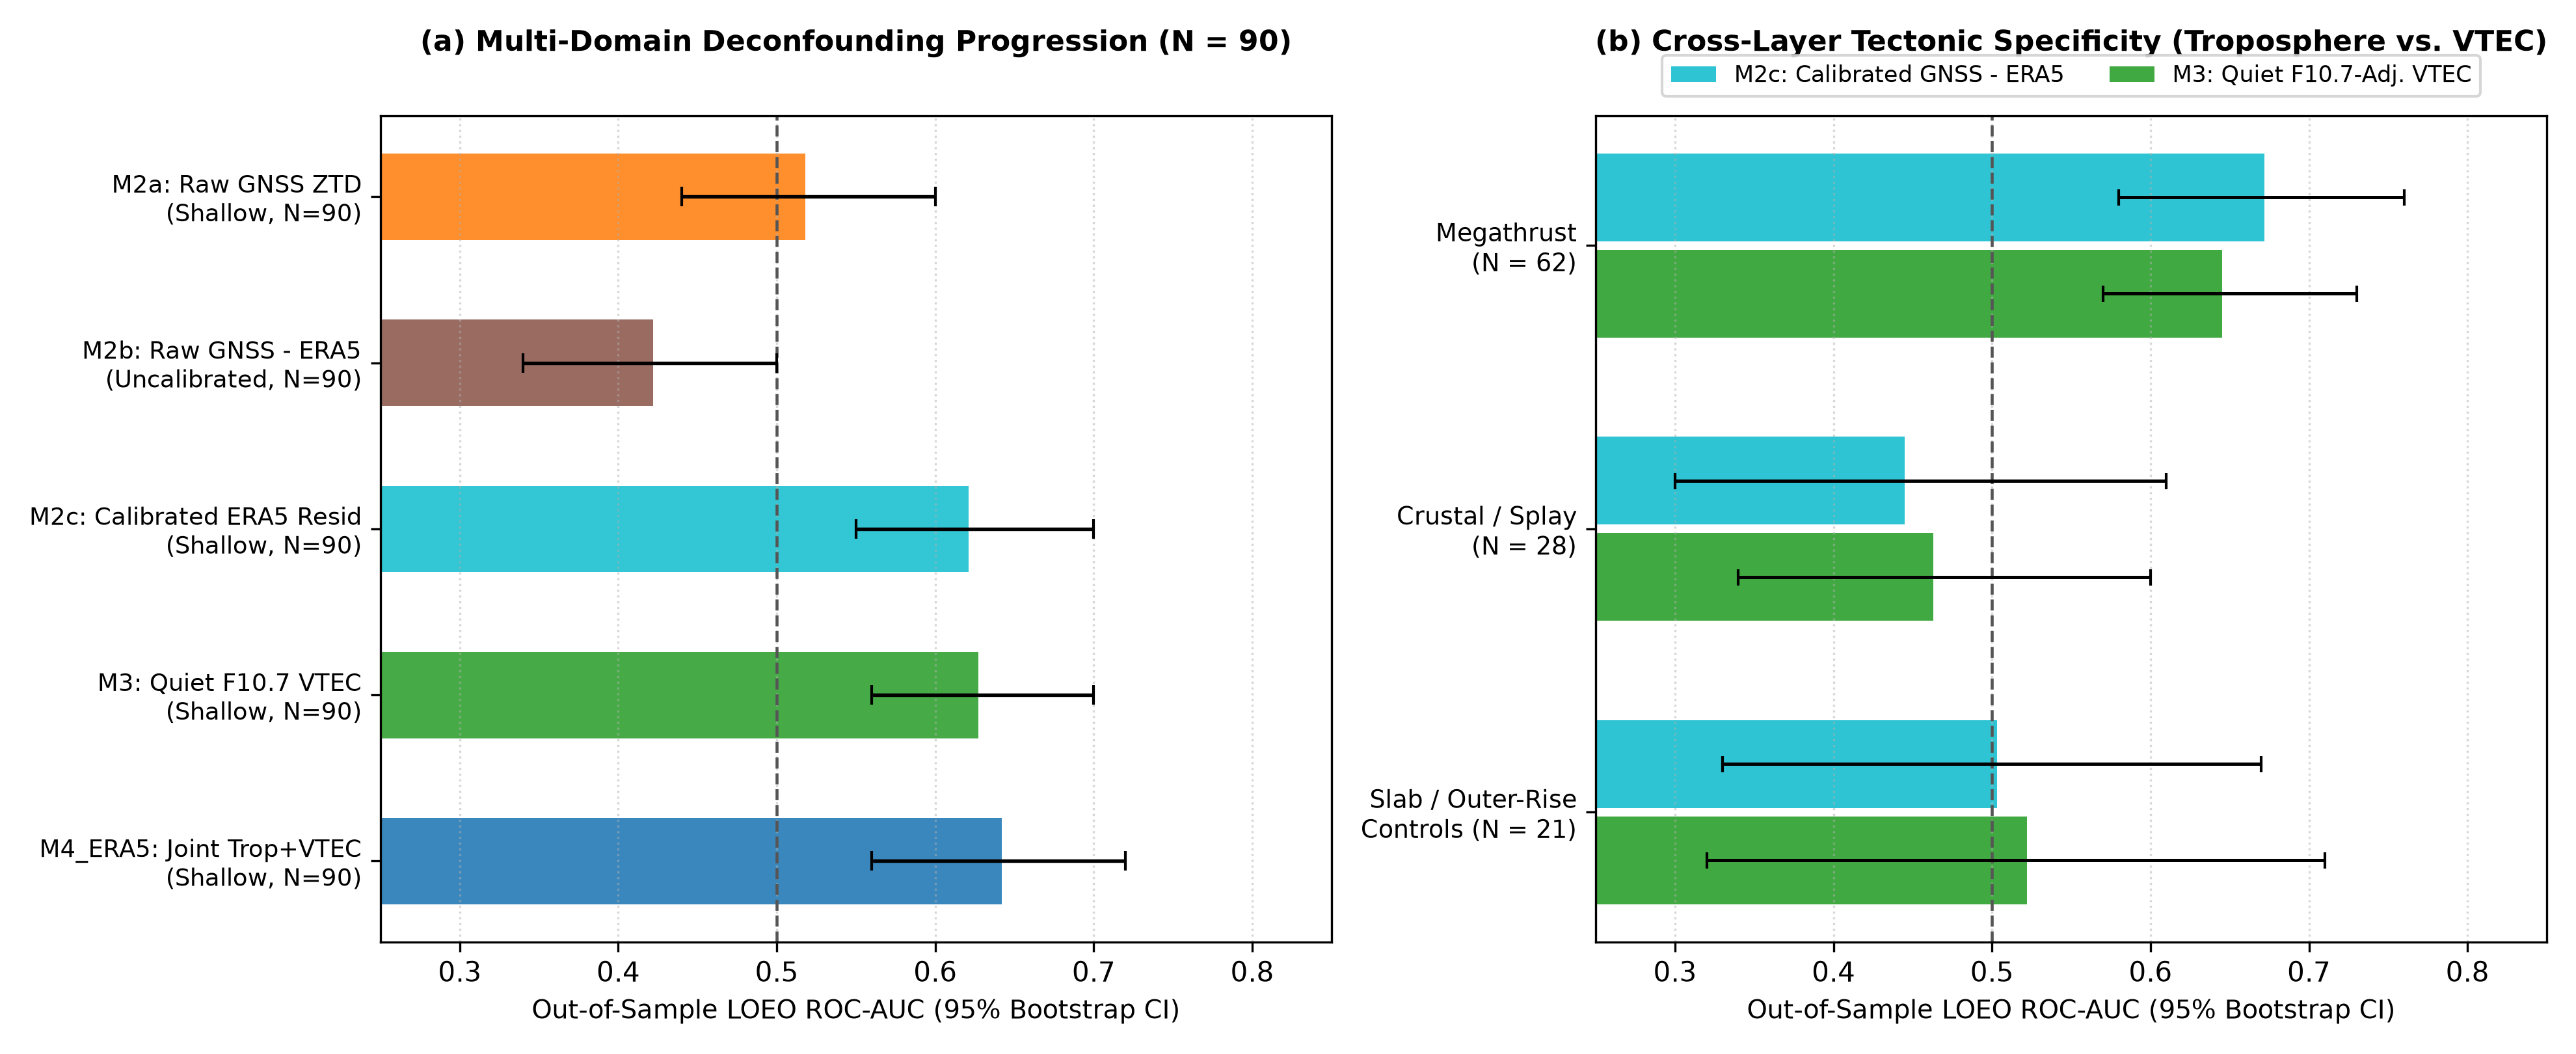
\includegraphics[width=0.96\textwidth]{figures/fig_stage5f_combined_benchmark.png}
\caption{LAIC-GUARD (\texttt{v002} + \texttt{v002\_era5}) zero-overlap, equal-lag ($1\text{--}10$\,d) out-of-sample $\text{ROC-AUC}$ with 95\% cluster-bootstrap confidence intervals across (a) progressive meteorological and ionospheric deconfounding models ($N = \LgPairedShallowMain$), and (b) tectonic mechanism and candidate negative-control strata.}
\label{fig:benchmark_v002_combined}
\end{figure*}

Raw GNSS ZTD ($\text{AUC} = \LgAucZtdRaw$) and uncalibrated $\text{GNSS} - \text{ERA5}$ differences ($\LgAucEraUncal$) fail to separate pre-seismic windows from placebo due to synoptic weather and $0.25^\circ$ grid-elevation mismatch. Applying station-specific linear transfer calibration within each causal baseline (M2c) isolates a non-meteorological ZTD residual ($\text{AUC} = \LgAucEraCal$, $p_{\text{Wilc}} = 0.0009$; $\LgAucEraCalCluster$ under $\pm 15$\,d storm-cluster CV). Independently, M2c and quiet $F_{10.7}$-adjusted VTEC (M3) converge on shallow megathrust interface earthquakes ($\text{AUC} = \LgAucEraMegathrust$ and $\LgAucVtecMegathrust$, $N=62$), while remaining indistinguishable from chance on crustal/splay ruptures ($\LgAucEraCrustal$, $\LgAucVtecCrustal$, $N=28$) and slab/outer-rise controls ($\LgAucEraNullCtrl$, $\LgAucVtecNullCtrl$, $N=21$). Fusing calibrated ERA5 residuals with quiet VTEC (M4$_{\text{ERA5}}$) yields $\text{AUC} = \LgAucJointEraVtec$.

\section{Limitations, Data Availability, and Conclusion}
While causal-window OLS calibration in M2c prevents future leakage, non-stationary synoptic shifts between baseline windows can influence residual variance; nonetheless, chance-level performance on slab controls ($\LgAucEraNullCtrl$) argues against a generic baseline artifact. Together, our findings show that meteorological and solar deconfounding isolates a modest, megathrust-specific multi-layer association rather than an operational earthquake-prediction capability. All benchmark manifests, verification scripts, and provenance ledgers (\texttt{tag: v002\_era5}) are openly available at \url{https://github.com/Parth15-git/LAIC-GUARD}.

\bibliographystyle{IEEEtran}
\bibliography{references}
\end{document}
